l\section{Results}
\label{sec:results}

In the following sections, we explore the response of the log-loss and Brier score metrics to the classifiers of Section~\ref{sec:data} and as a function of the weights on affected classes.

\subsection{Mock classifier systematics}
\label{sec:mockresults}

\begin{figure*}
	\begin{center}
		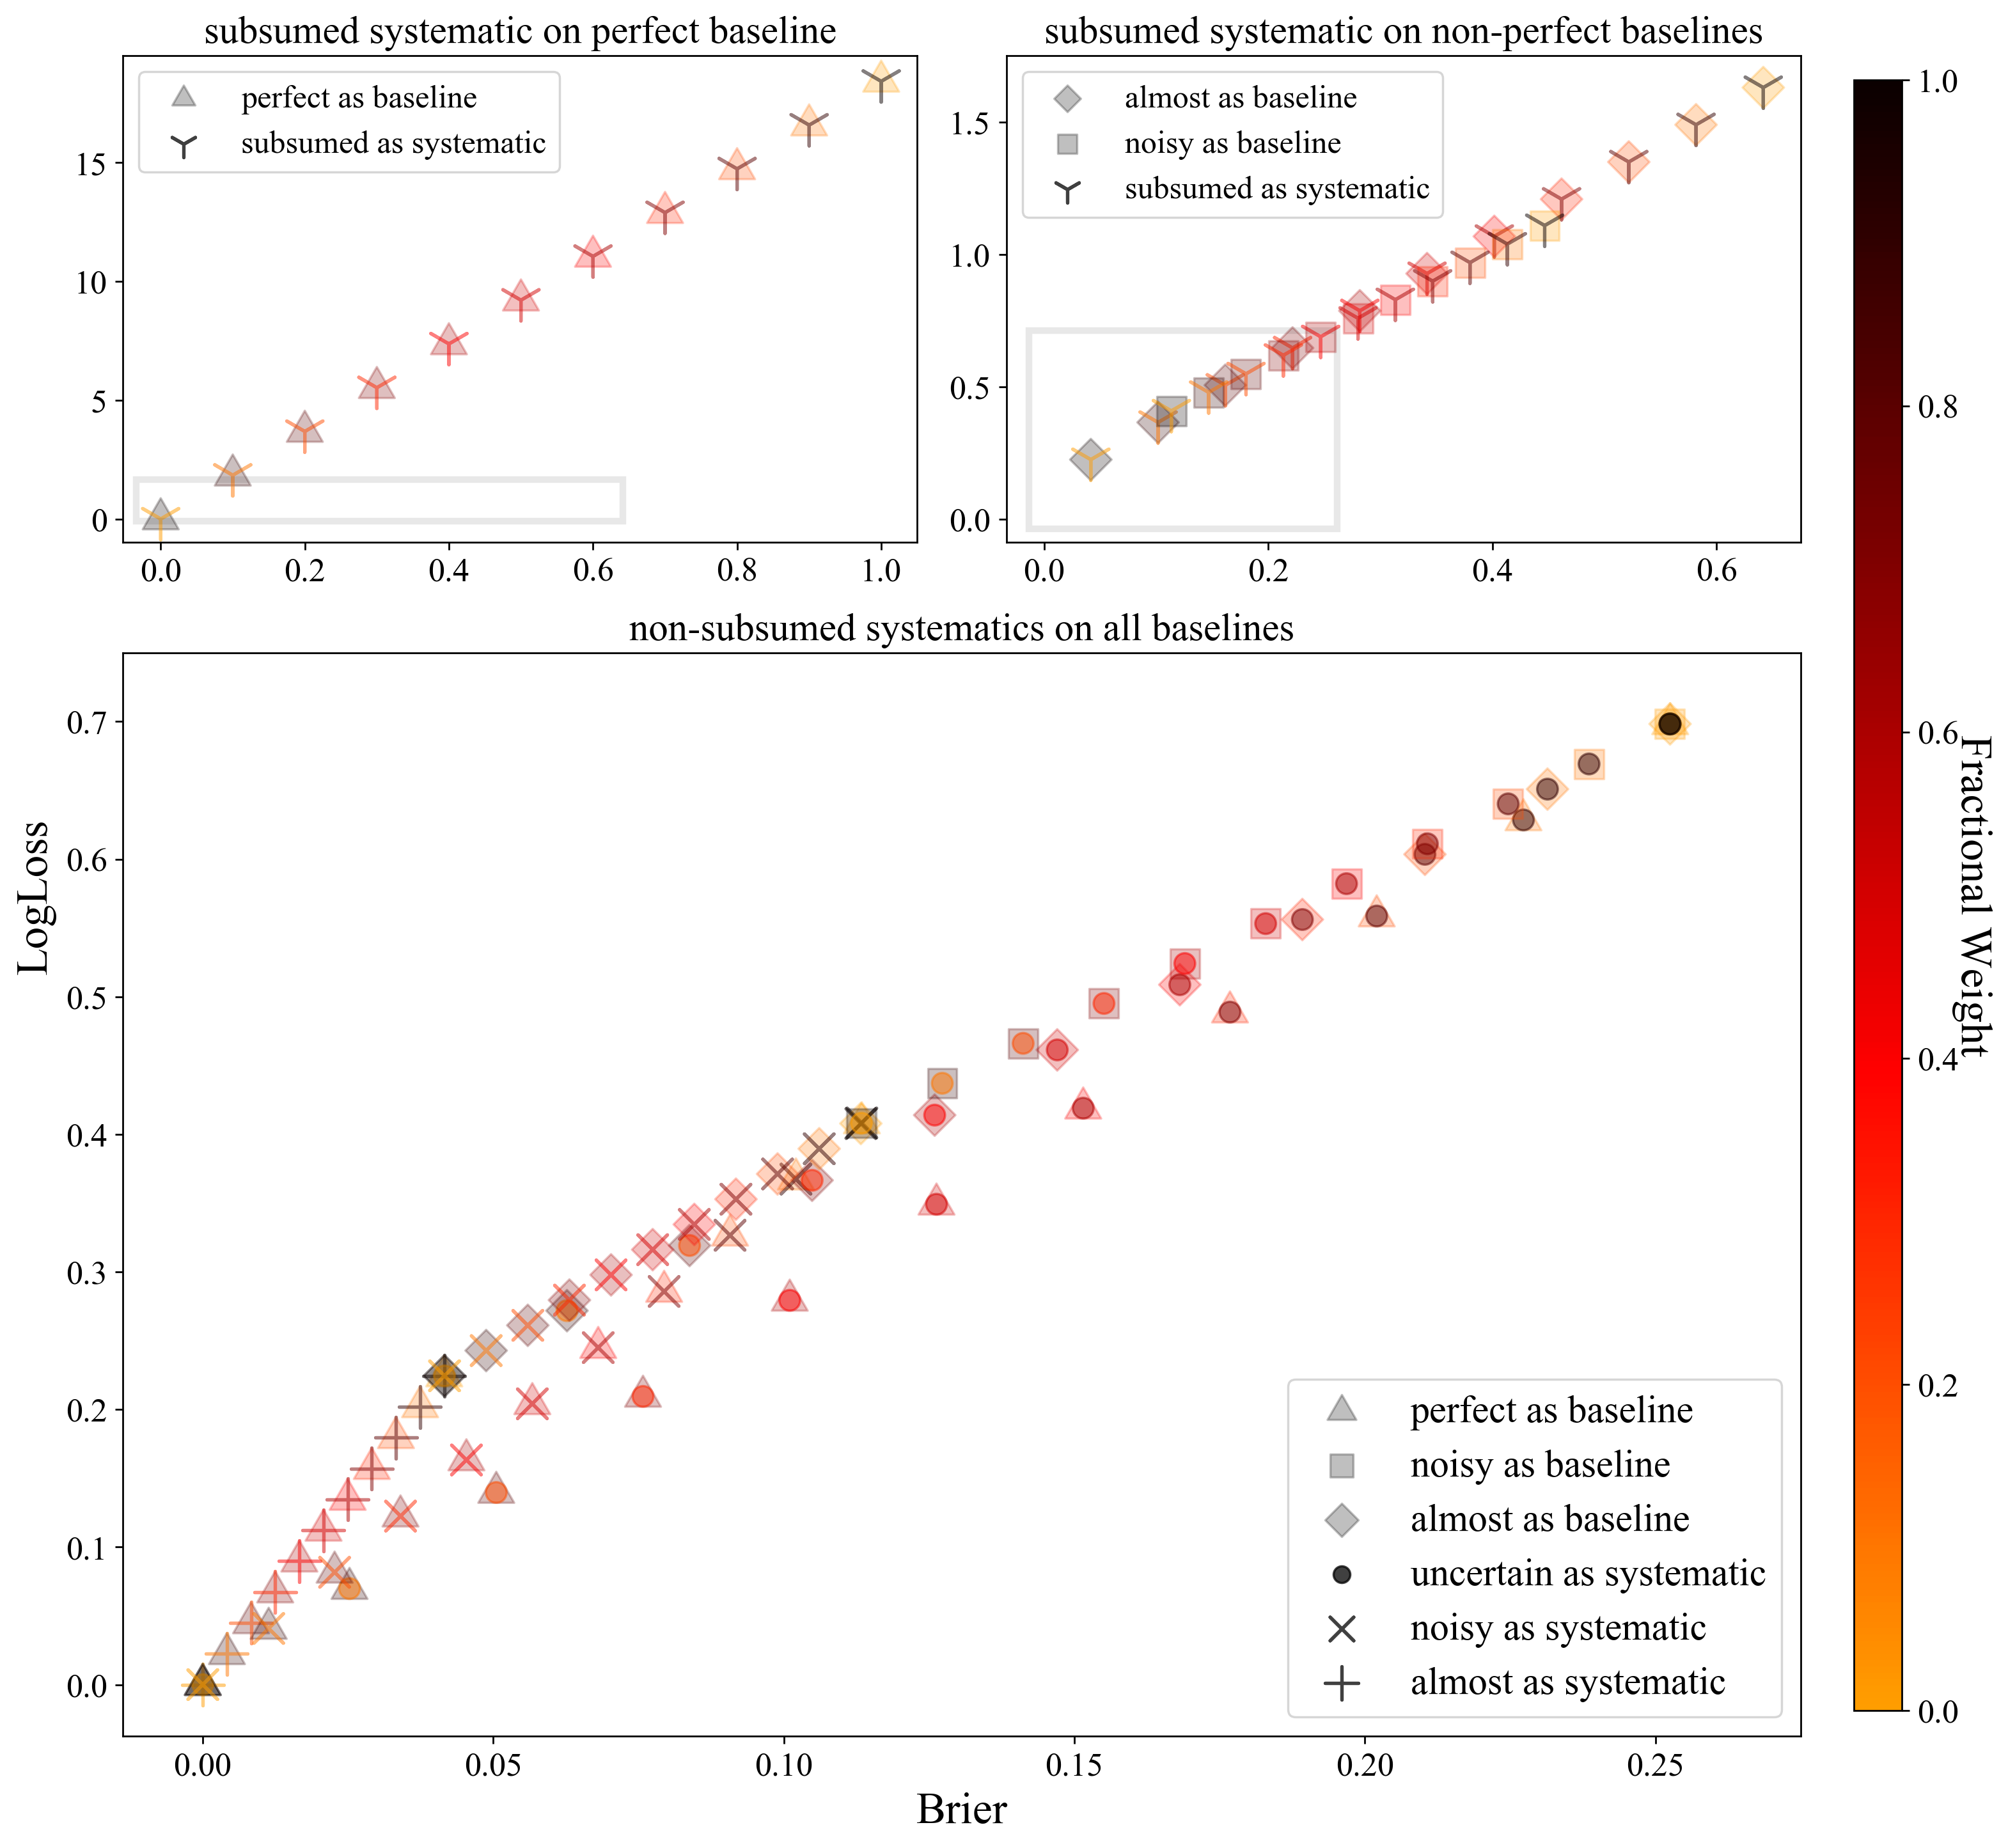
\includegraphics[width=0.99\textwidth]{./fig/multipanel_res.png}
		\caption{Weighted log-loss and Brier scores for baseline classifiers with combinations of systematics.
		Each point represents a classifier with baseline behavior (classifiers with perfect behavior are shown as triangles, noisy classifiers are shown as squares and almost perfect classifiers as diamonds). The asterisk markers show the case where one class is given a systematic effect. From left to right, we zoom in on a particular range of Brier/log-loss scores, to highlight the effect of systematics on the scores for well-behaved methods with low Brier/log-loss scores. 
		The color of the marker for the systematic effect indicates the weight on the one class affected by that systematic, while the color of the baseline behavior marker indicates the integrated weight evenly distributed over other classes with baseline behavior. The `subsumed as' systematic on a perfect baseline (triangle with `y-shaped' marker) is the classification example that is most sensitive to changes in the class weight, as can be seen by the changes in log-loss score in the left hand panel.
%		Both metrics are shown in three regimes of sensitivity: to the subsumed systematic on a perfect baseline is highest, all other baselines with the subsumed systematic, and all other systematics.
		The ranges of Brier score and log-loss values between the panels are in ratios of approximately 10:7:3 and 100:10:5, respectively, indicating the log-loss's higher sensitivity to the presence of systematics.
		}
	\end{center}
	\label{fig:all_combined}
\end{figure*}
We simulate entries to the \plasticc\ classification challenge by generating random draws of the combined CPM (composed of classififiers with different systematics) described in Section~\ref{sec:mockdata} is shown in Figure~\ref{fig:all_combined}.

The systematics introduced to each baseline are those that we intuitively expect to worsen classification performance of an arbitrary classifier:
\begin{itemize}
\item the uncertain, almost perfect, noisy, and subsuming classifiers are anticipated to worsen an otherwise perfect classifier;
\item the uncertain, noisy, and subsuming classifiers are anticipated to worsen an otherwise almost perfect classifier;
\item the uncertain and subsuming classifiers are anticipated to worsen an otherwise noisy classifier.
\end{itemize}

In every case, we apply the systematic to one true class, i.e. transforming one row of the baseline conditional probability matrix.
The metrics are evaluated at a number of weights $w$ on the affected class, with the weights on the remaining baseline classes equal to one another at $(1 - w) / (M - 1)$.

%The weight values range from $0$ (all weight on the baseline) to $1$ (all weight on the systematic) at intervals of $0.1$.
%This variation in weights establishes linear relationships between the log-loss and Brier score metrics for each pair of baseline and systematic.

%Figure~\ref{fig:all_combined} confirms that for all weights on the perfect classifier, the values of both metrics vanish to zero.
%It is immediately evident that the log-loss has more dynamic range than the Brier score overall, and that the log-loss is acutely sensitive to the subsuming systematic on a baseline of a perfect classifier.
%In fact, the log-loss value for a classifier that subsumes a class into one that is classified perfectly should actually be infinite if the classes unaffected by the systematic have no weight.
%The finite maximum in our tests is set by the artificial zero point established for numerical stability.
%Because the combination of a subsuming classifier with a perfect baseline (left panel) is so different from all other combinations, we separate the subsuming systematic on all other baselines (middle panel) from all other systematics (right panel) in Figure~\ref{fig:all_combined}.
%The dynamic range of the log-loss remains higher even outside the regime where it tends toward infinity.
%The extent of the values of both metrics is higher in the middle panel with the subsuming systematic on various baselines than in the right panel with all other systematics.
%This shows that both metrics are still more sensitive to the subsuming systematic than any other systematic, confirming that both can appropriately penalize the cruise control effect.

In Figure~\ref{fig:all_combined}, we show the overall performance of a given classification algorithm, but highlight how the classification performance of one class changes the combined metric. In every case, we apply the systematic to one true class at a time, i.e. transforming one row of the baseline conditional probability matrix. 
In order to illustrate the effect each particular systematic has on a given class, and more importantly, how up- (or down-) weighting that class changes the overall performance of the classification algorithm, we evaluate the metric at a number of weights $w$ on the affected class, with the weights on the remaining (baseline/unaffected) classes equal to one another at $(1 - w) / (M - 1)$.
%The metrics are evaluated 
The weight values range from $0$ (all weight on the baseline classes) to $1$ (all weight on the class affected by the systematic) at intervals of $0.1$, as shown in Figure~\ref{fig:all_combined}. The more a class affected by the systematic is weighted (shown by baseline markers that are more green, with systematic indicators that are more blue in color), the more the log-loss and Brier scores increase -- the classifications fare poorly in these metrics. The left-most plot shows the largest variations in metric scores, for the combination of perfect baselines (all but one class are perfect) and a `subsumed as' systematic where another class is consistently misclassified into the systematic class. 

This variation in weights establishes linear relationships between the log-loss and Brier score metrics for each pair of baseline and systematic. In addition, Figure~\ref{fig:all_combined} confirms that for all weight on the perfect classifier, the values of both metrics vanish to zero. It is worth noting that the log-loss has more dynamic range than the Brier score overall, and that the log-loss is acutely sensitive to the subsuming systematic on a baseline of a perfect classifier. In fact, the log-loss value for a classifier that subsumes a class into one that is classified perfectly should actually be infinite if the classes unaffected by the systematic have no weight.

The middle plot illustrates a narrower range of log-loss and Brier scores for two baseline scenarios: almost perfect and noisy.
In both cases, the systematic effect shown is again `subsumed as', and the relationship between the weight of the systematic and the weight of the baseline is again roughly linear with a large slope. 
The slope of the line is smaller in the third panel, where a range of baselines and of systematics are shown. This highlights that both the log-loss and Brier scores are most sensitive to the subsuming systematic than any other systematic, and that strongly up-weighting one particular class has a detrimental affect on the global performance of a classifier.
\textbf{[RH added the above to make sure that folks take away two messages: weighting objects with a particular systematic can dramatically change your result for both metrics; and the log-loss is a bit more sensitive to systematics than the Brier - penalising them.}

%  confirming that both can appropriately penalize the cruise control effect.

%%The finite maximum in our tests is set by the artificial zero point established for numerical stability.
%Because the combination of a subsuming classifier with a perfect baseline (left panel) is so different from all other combinations, we separate the subsuming systematic on all other baselines (middle panel) from all other systematics (right panel) in Figure~\ref{fig:all_combined}.

%The extent of the values of both metrics is higher in the middle panel with the subsuming systematic on various baselines than in the right panel with all other systematics.



\begin{table}[]
\begin{tabular}{lll}
Classifier characteristic & Brier score & Log-loss\\
\hline
Perfect & 0.0 & 0.0\\
Almost perfect & 0.042 & 0.225\\
Noisy & 0.113 & 0.408\\
Uncertain & 0.253 & 0.699\\
Subsumed from Noisy & 0.447 & 1.109\\
Subsumed from Almost & 0.641 & 1.629\\
Subsumed from Perfect & 1.0 & 18.421\footnote{The entry for the log-loss of a classifier that subsumes a class into one that is otherwise perfectly classified should be infinite but is bounded by the numerical precision of our calculations.}
\end{tabular}
\caption{Weighting changes the metric performance: the value of each metric when the weight is entirely on the class(es) with the indicated characteristic (correponsding to a $w=1$ case in Figure~\ref{fig:all_combined}). The log-loss is more sensitive than te Brier score, with larger values of the score (indicating poor classification performance), particularly for the subsumed from systematics.}
\label{tab:extents}
\end{table}

When all weight is on the class affected by a systematic, there is a characteristic limit for each metric's values, shown in Table~\ref{tab:extents}. Because a subsumed class takes the conditional probability vector of the subsuming class, the metric values depend on what systematics may be affecting the subsuming class as well. While the precise values of the scores are not equal (the slopes between the two metrics are given in Table~\ref{tab:slopes}), the two metrics rank the classification scenarios in the same order. 
In general, one would hope for metrics that exhibit this behaviour, but this is not guaranteed.

%Based on Table~\ref{tab:extents}, both metrics would agree on the ranking of these classifiers, though this agreement is not in general guaranteed.

%Furthermore, this invariant ranking is consistent with our intuition about the severity of anticipated faults of classifiers.

\begin{table}[]
\begin{tabular}{l|llll}
	& Systematics & & &\\
Baselines & Subsumed & Uncertain & Noisy & Almost\\
\hline
Perfect & 18.421 & 2.763 & 3.601 & 5.387\\
Almost perfect & 2.343 & 2.246 & 2.556 & \\
Noisy & 2.102 & 2.085 & &
\end{tabular}
\caption{The slopes for each baseline-plus-systematic pair in the space of log-loss versus Brier score.
A higher slope corresponds to increased sensitivity of the log-loss.}
\label{tab:slopes}
\end{table}

The relative sensitivity ratios of the log-loss to the Brier score are the slopes in the trends of Figure~\ref{fig:all_combined} and are given in Table~\ref{tab:slopes}.
The log-loss always has higher sensitivity than the Brier score (i.e. it responds more strongly to up-weighting classes whose clasification displays a systematic), particularly to the difference between the perfect classifier and any lesser classifier.
A possible implication of this behavior is that the log-loss may have an enhanced ability to distinguish between multiple high-performing classifiers that might not have meaningfully different metric values under the Brier score.

On the other hand, the log-loss is more susceptible to the tunnel vision classifier \textbf{[RH: why? this isn't clear - link this to weights discussion earlier]}, with a significant response to any move toward perfection.
Now that we have investigated how the metrics respond to idealized classifications with known/expected systematics, we can investigate the performance of both the Brier metric and the log-loss metric on a more representative classification method as applied in an astronomical context.
% Heavily unequal weighting can incentivize tunnel vision classification.
% However, the slope is higher for the almost perfect systematic than the noisy systematic, and higher for the noisy systematic than the uncertain systematic; this means that a tunnel vision classifier is deprived of the metric's favor more if it neglects other classes than if it already does fairly well for them, a case in which we would not call it much of a systematic.

% \aim{Still reworking past here.}
% Consider a weighting of $\sim0.8$ for a class affected by tunnel vision, leaving $\sim0.2$ to be shared evenly among all other classes uniformly affected by the other systematics.
% Qualitatively, we would say that a classifier that is almost perfect for other classes is superior to one that is noisy, and a classifier that is noisy for other classes is still superior to one that is uniform; furthermore, the subsuming classifier is even more harshly penalized in this situation than the uncertain classifier, meaning both metrics are  consistent with our basic tests of intuition in this case.
% However, this observation also indicates that the tunnel vision systematic is difficult to penalize, and that if the affected class is given a large weight, it can easily dominate the metric.
% If all classes are of scientific importance, heavily unequal weighting can incentivize tunnel vision classification.

% We introduced weighting of per-class metrics to discourage `tunnel vision' and `cruise control' classifiers that can ignore classes other than the most common and nonetheless perform well by a metric.
% Figure~\ref{fig:popweight} shows the impact of weighting the per-class metrics by the number of objects in the class as each is affected by one of the systematics and the other classes are held at the more realistic almost perfect performance.
% The points show different classification schemes, and all points are coloured by the change in the weighting, dependent on the size of the population class being classified.
% Conversely, the cruise control classifier and, to a lesser degree the noisy classifier, always has high log-loss and Brier score values regardless of the weight on the affected class.

% \begin{figure}
% 	\begin{center}
% 		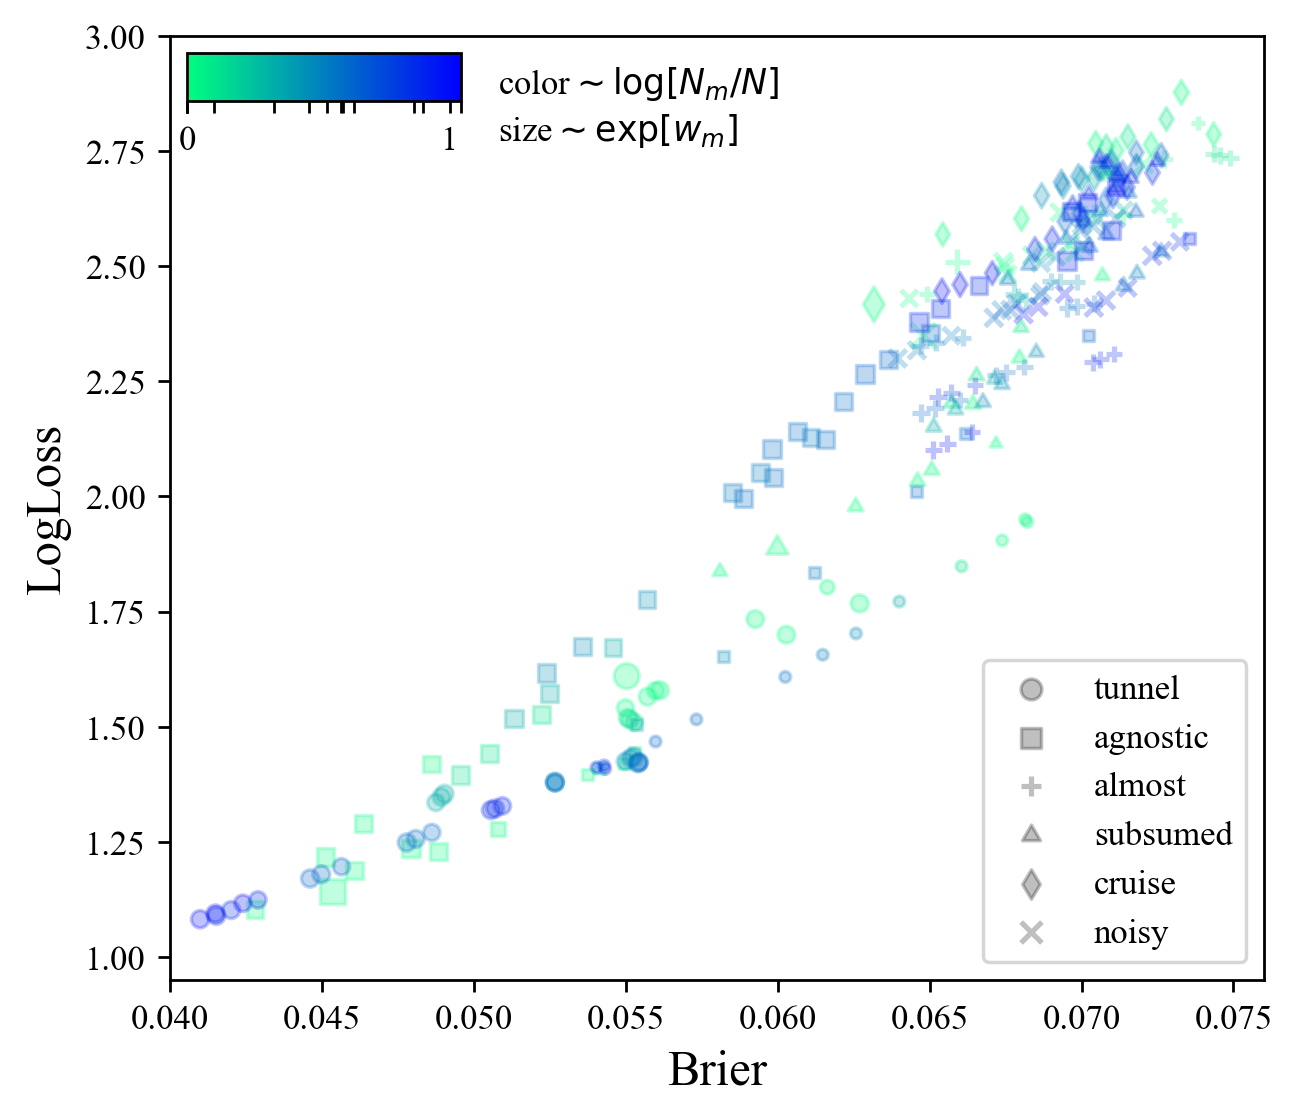
\includegraphics[width=0.5\textwidth]{./fig/all_effects_isolated.png}
% 		\caption{Population-weighted log-loss and Brier scores for classifiers with one class affected by a systematic, as a function of the population of the affected class.
% 		Each point corresponds to an almost perfect classifier that with one class instead affected by a systematic (shape), with log-loss on the $y$ axis and Brier score on the $x$ axis.
% 		The metrics are calculated with a weighting (color and size) proportional to the log of its weight in a weighted average following Equation~\ref{eq:weightavg}.
% 		}
% 	\end{center}
% 	\label{fig:popweight}
% \end{figure}

% The tunnel vision classifier has a consistently low value under the Brier score and log-loss metric (bottom left corner of the plot), only increasing its Brier score once the weighting drops (less blue).
% In this view, the Brier score appears to be more susceptible to tunnel vision than the log-loss, demonstrating a more significant decrease as the size of the affected class increases, but both metrics have concerning behavior in this regard.
% This finding suggests that weighting alone may not be sufficient to counter the influence of this effect, and indicates a need for another balancing mechanism, such as requiring a threshold metric value on all classes.
% When considering a method of converting from one of these metrics to a finall `winner' of the classification challenge, care must be taken to ensure that all approaches do reasonably well at classifying more than one object.
% This thresholding procedure is discussed in the text

% \textbf{Ashish to reaplce/add more here?}
%\aim{Preliminary results indicate weighting will be very important for preventing the tunnel vision classifier from winning. It may be necessary to a priori anticipate which classes will have to be most strongly protected from this systematic via upweighting them.}

%\begin{figure}
%	\begin{center}
%		% 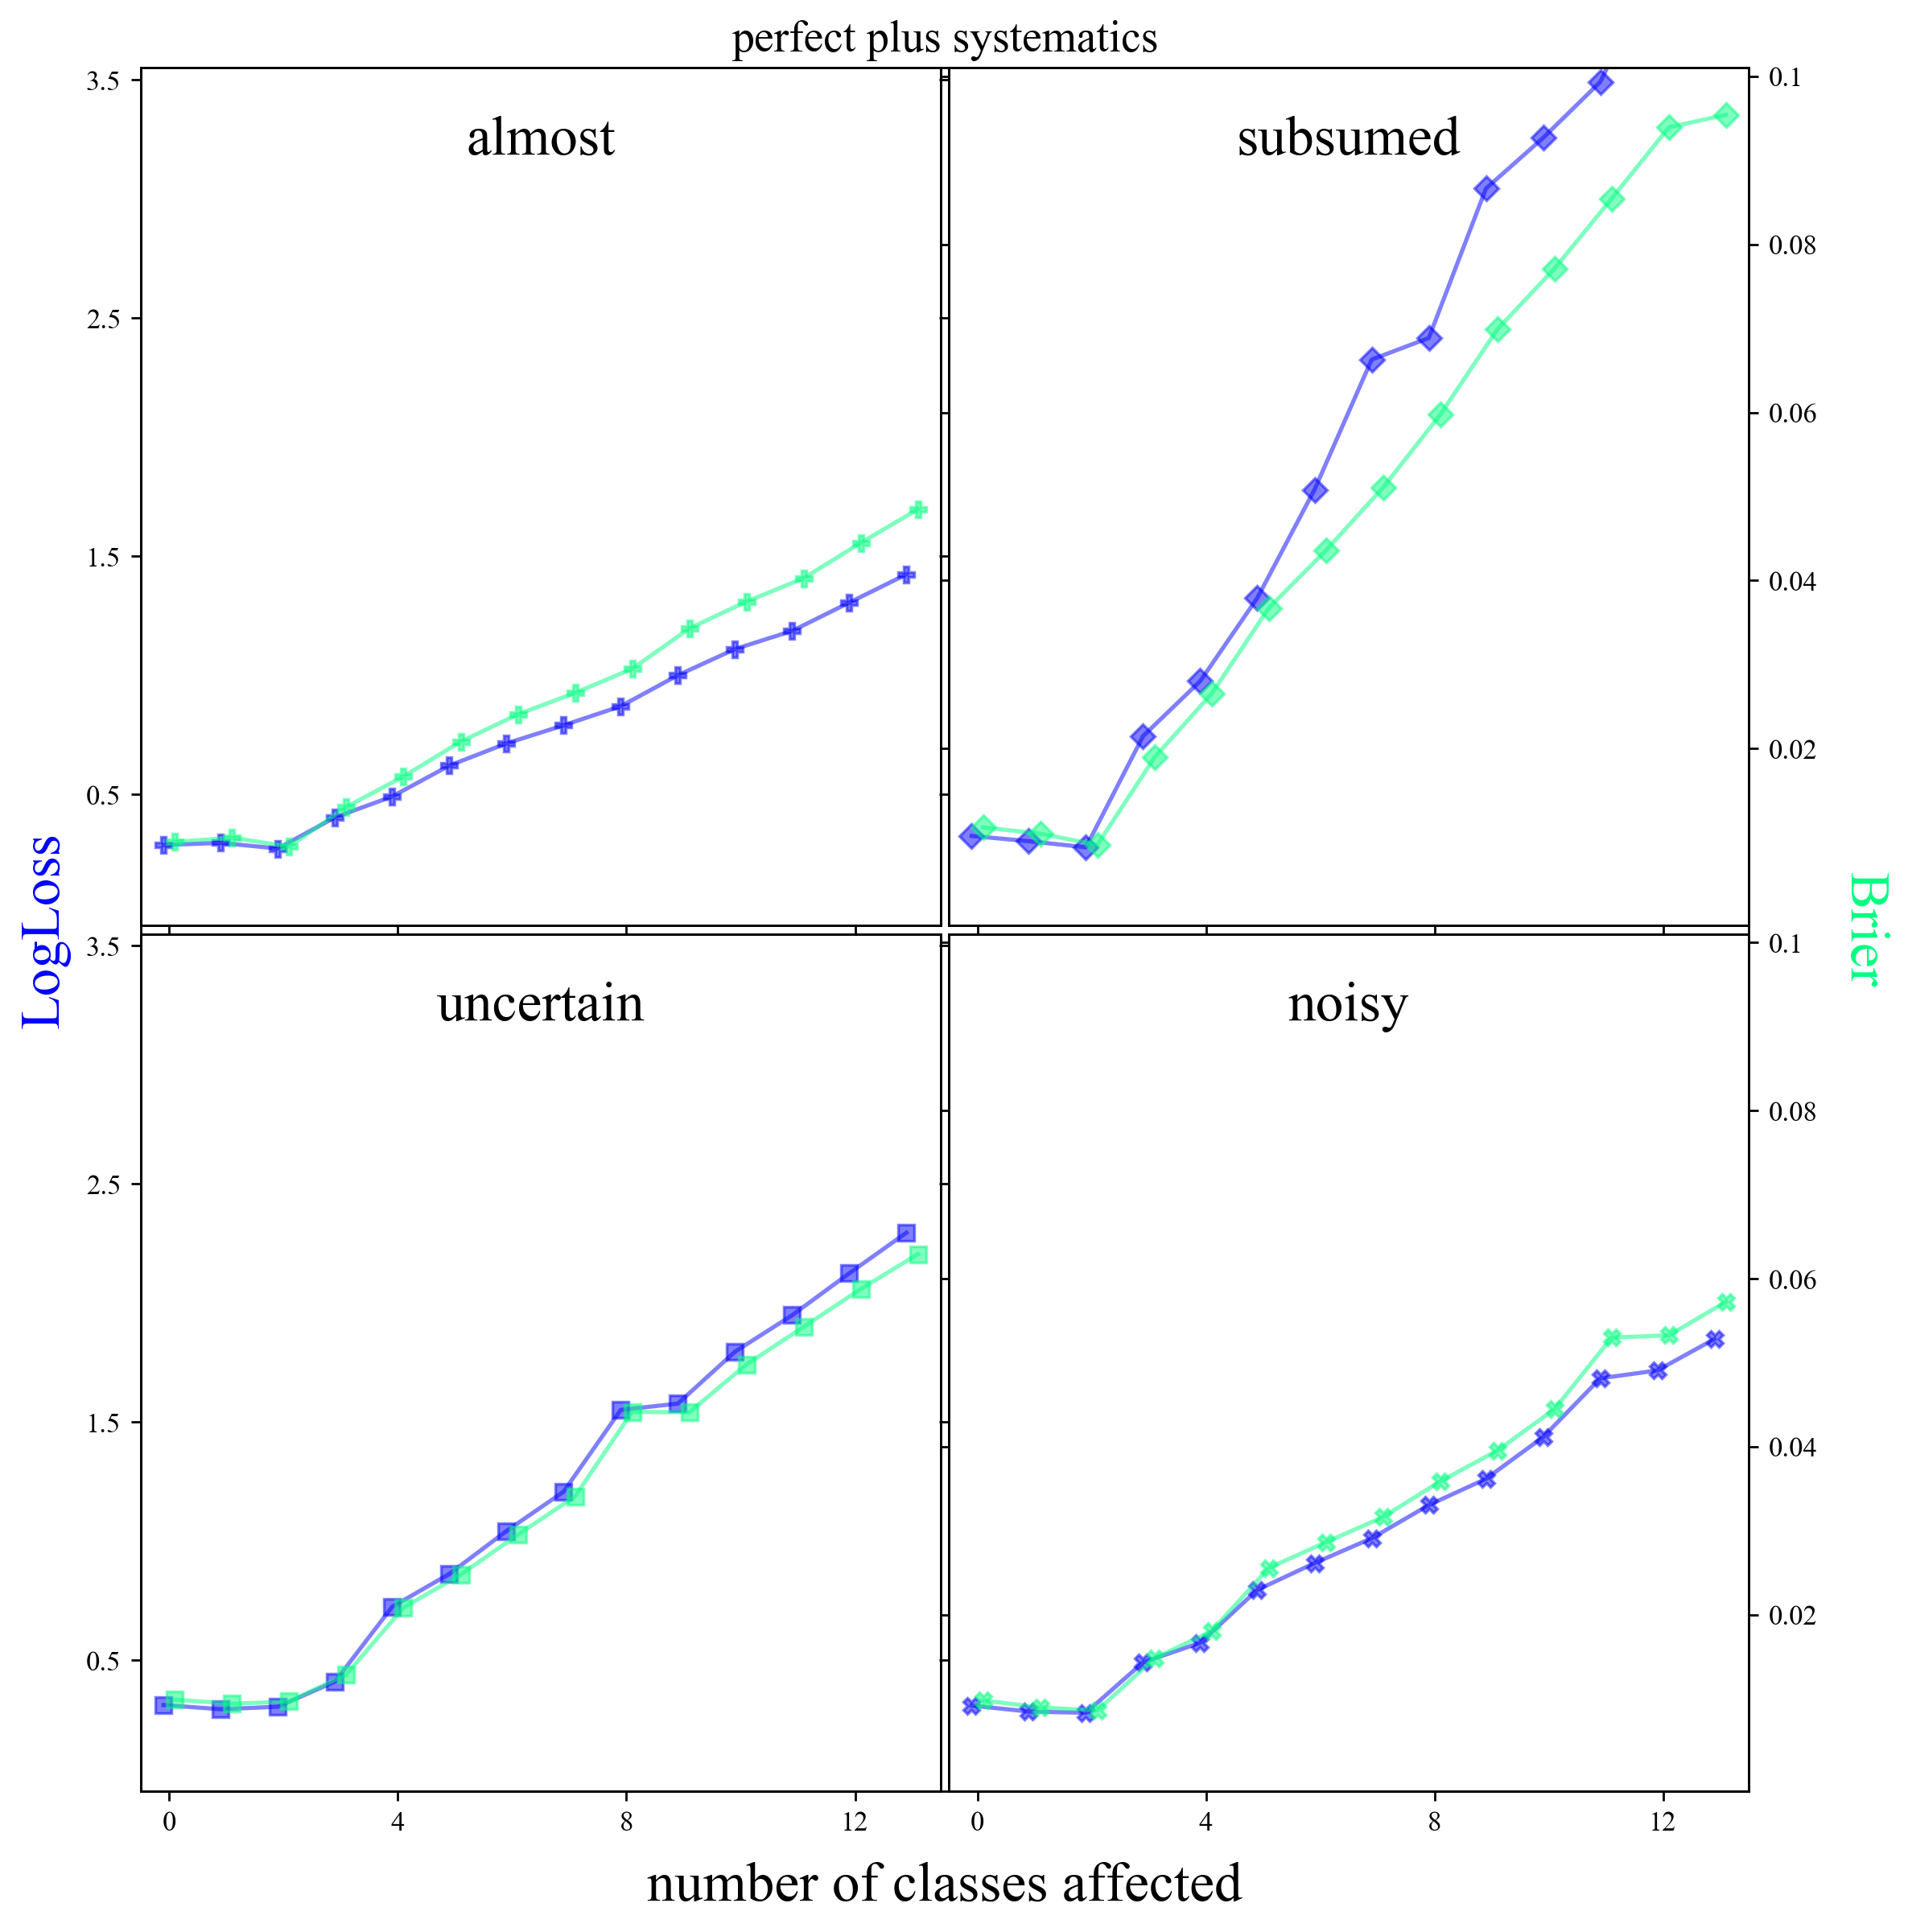
\includegraphics[width=0.5\textwidth]{./fig/systematics_onlyperfect.png}
%		\caption{\aim{After much iteration on how best to present these tests, a figure similar to Figure~\ref{fig:cruise} but for the tunnel vision classifier (heading) on different baseline classifications (panels) as a function of weight on the affected class (rather than number of classes) is under construction.}}
%		\label{fig:tunnel}
%	\end{center}
%\end{figure}

\subsection{Representative classifications}
\label{sec:realresults}
We apply the log-loss and Brier metrics to the classification output from \textsc{snmachine}. While the classification methods described in \citet{lochner_photometric_2016} refer to the idealized subset of the \snphotcc\ data, these approaches are the state-of-the-art in classification of extragalactic transients. We present in Table~\ref{tab:snmachineresults} the log-loss and Brier scores assuming an equal weight per object. 
%, for classification probabilities derived from running the algorithms of \citet{lochner_photometric_2016} on the \snphotcc\ data of Section~\ref{sec:realdata}.
Table~\ref{tab:snmachineresults} also contains the ranking of classifier performance under each metric.


\begin{table*}[]
	\begin{centering}
\begin{tabular}{lllllll}%ll}
Rank $R$ & $R_\mathrm{FoM}$ & FoM & %$R_\mathrm{AUC}$ & AUC &
$R_\mathrm{LogLoss}$ & Log-loss & $R_\mathrm{Brier}$ & Brier \\
\hline
1  & TBDT & 0.635  %& TBDT & 0.982
& TBDT & 0.0907 & TBDT & 0.0486 \\
2  & WBDT & 0.591  %& WBDT & 0.978
& TSVM & 0.113  & TSVM & 0.0583 \\
3  & TSVM & 0.514  %& TSVM & 0.969
& TNN  & 0.125  & TNN  & 0.0650 \\
4  & WSVM & 0.499  %& WSVM & 0.968
& WSVM & 0.1316 & WBDT & 0.0689 \\
5  & TNN  & 0.496  %& TNN  & 0.954
& WBDT & 0.1321 & WSVM & 0.0730 \\
6  & WNN  & 0.480  %& WNN  & 0.946
& TKNN & 0.146  & WNN  & 0.0750 \\
7  & TKNN & 0.384  %& TKNN & 0.942
& WNN  & 0.152  & TKNN & 0.0787 \\
8  & TNB  & 0.340  %& WKNN & 0.894
& WKNN & 0.228  & TNB  & 0.105  \\
9  & WKNN & 0.114  %& TNB  & 0.879
& TNB  & 0.251  & WKNN & 0.132  \\
10 & WNB  & 0.0365 %& WNB  & 0.850
& WNB  & 0.443  & WNB  & 0.178  \\
\end{tabular}
	\caption{Metric performance: the values of three metrics for each of ten \snmachine\ classifiers with equal weight per object.
	The metrics broadly agree on the ranking of the classifiers, confirming consistency between a conventional metric of classification performance and the metrics of probabilistic classifications presented here.
	However, there are some differences with pairwise swapping between the log-loss and Brier rankings and some significant reordering of ranks 2 through 5 with the FoM metric relative to the probabilistic metrics.}
	\label{tab:snmachineresults}
	\end{centering}
\end{table*}

For the first- and last-ranked methods, the Brier and log-loss scores are in agreement. 
The FoM for the \snphotcc\, as described in Section~\ref{sec:science} differs more from the Brier and log-loss metrics than they do from one another. This is perhaps not that surprising, given that the \snphotcc\ was specifically looking to value classification algorithms that were pure (that yielded a large number of SNIa classifications and few interlopers from the other classes), as opposed to metric that rewards good performance across classes. All three metrics are in agreement over the winners and losers, indicating that both of the potential \plasticc\ metrics are roughly consistent with our intuition about what makes a good classifier. One should be careful not to generalize howwver, thee classifiers do not agree with one another on the entire ranking and could thus potentially disagree about the winner.

